\documentclass[10pt,twocolumn]{article}
\usepackage[margin=0.68in,columnsep=0.24in]{geometry}
\usepackage[T1]{fontenc}
\usepackage[utf8]{inputenc}
\usepackage{lmodern}
\usepackage{microtype}
\usepackage{amsmath,amssymb,amsthm}
\usepackage{booktabs}
\usepackage{graphicx}
\usepackage{xcolor}
\usepackage{enumitem}
\usepackage{hyperref}

\hypersetup{
  colorlinks=true,
  linkcolor=blue!60!black,
  citecolor=blue!60!black,
  urlcolor=blue!60!black,
  pdftitle={Certified Verification of Polynomial Decompositions, Discrete Tomography Reconfiguration, and Legendre Cross-Polytope Slice Integrals},
  pdfauthor={Lluis Eriksson}
}

\newtheorem{proposition}{Proposition}

\title{\vspace{-1.1em}\textbf{Certified Verification of Polynomial Decompositions, Discrete Tomography Reconfiguration, and Legendre Cross-Polytope Slice Integrals}}
\author{Lluis Eriksson\thanks{Independent Researcher. Code, Lean~4 proofs, and certificates: MIT License; manuscript and figures: CC-BY-4.0. Prepared with AI coding, formalization, and drafting assistance from Google Antigravity; all proofs, exact rational/integer verifiers, and adversarial tests were independently compiled and verified locally. Repository: \url{https://github.com/lluiseriksson/polynomial-decomposition-reconfig-certificates}}}
\date{November 25, 2026}

\begin{document}
\maketitle
\vspace{-1.4em}

\begin{abstract}
Peter Keevash and Jeck Lim (\texttt{arXiv:2611.33120}, Nov.\ 2026) resolved polynomial-time reconfiguration and approximate counting for discrete tomography and general $k$-directional integer matrices via $m$-basic polynomial decompositions in $\mathbb{Z}[x]$ (Thms.~1.1--1.4), a filling-norm lower bound using the witness family $F_{a,b,ab}(x) = (1-x^a)(1-x^b)-(1-x)(1-x^{ab})$ (Prop.~3.7), cyclotomic divisibility (Sec.~4.1), and a ``miraculous'' exact global polynomial theorem for weighted Legendre cross-polytope slice integrals $R_l(r,s)$ (Thm.~1.6). We construct a standalone zero-dependency \textbf{Lean~4.35.0} formalization of 18 core tomography, $\mathbb{Z}[x]$-ring, Proposition~3.7 Cramer-elimination, Legendre/Murphy, Theorem~1.6 global slice-integral, and cyclotomic-factorization theorems (zero \texttt{sorry}, zero warnings, zero \texttt{Classical.choice}) paired with a zero-floating-point exact $\mathbb{Q}/\mathbb{Z}$ verifier (\texttt{POLY-DECOMP-CERT-1.0}). Across 16 canonical certificates ($0.062$--$2.740\,\mathrm{ms}$, total $8.07\,\mathrm{ms}$), all exact Legendre slice polynomials, $m$-basic decompositions, multi-direction tomography switches, and filling-norm witnesses replay deterministically while rejecting 60/60 live adversarial forgery attacks.
\end{abstract}

\section{Introduction}\label{sec:intro}
Efficient reconfiguration and approximate counting of integer matrices with prescribed projections---classical contingency tables~\cite{diaconis1998algebraic,dyer1997sampling,barvinok2010number}, transportation polytopes~\cite{deza2010diameter}, and discrete tomography~\cite{gardner1999discrete,hajdu2001algebraic}---hinge on decomposing zero-projection differences into elementary switches of bounded support. Keevash and Lim~\cite{keevash2026efficient} established a general algebraic framework with four central mechanisms:
\begin{enumerate}[leftmargin=*,nosep]
  \item \textbf{Miraculous Legendre Slice Integrals (Thm.~1.6, Sec.~1.4 \& 2.1):} Weighted by Murphy's Legendre polynomial $L_{k-1}$~\cite{szego1939orthogonal}, the cross-polytope slice integral $R_l(r,s)$ simplifies globally to a degree-$(k-1)$ polynomial satisfying $R_l(-r,-s)=R_l(s,r)=R_l(r,s)$ and exact constant marginal $\int_{-1}^1 R_l(r,s)\,ds = 2/k!$ despite $3k(k-1)/2 > k$ overdetermined symmetry constraints.
  \item \textbf{$m$-Basic Polynomial Decompositions (Thms.~1.2 \& 1.4):} Reducing multi-directional switches via determinant projections maps zero-X-ray grids to integer polynomials divisible by $(1-x)^k$, decomposed into sums of $m$-basic atoms $\pm x^a \prod_{i=1}^k (1-x^{m_i a_i})$ with controlled $L^1$ norm.
  \item \textbf{Discrete Tomography Reconfiguration (Sec.~1.1, Thm.~1.1):} Multi-directional basic switches annihilate X-ray projections $\pi_v$ along every primitive lattice direction $v = (a,b)$ via the line invariant $bx - ay$, enabling bounded-entry reconfiguration paths between equal-X-ray grids.
  \item \textbf{Filling-Norm Lower Bound \& Cyclotomics (Prop.~3.7, Sec.~4.1):} The witness $F_{a,b,c}(x) = (1-x^a)(1-x^b)-(1-x)(1-x^c)$ is divisible by $(1-x)^3$ iff $ab = c$, yields $4m+3$ monomial-matching equations in $4m$ variables, and resists small decompositions via base-$t$ Cramer non-vanishing; general $m$-weights factor through cyclotomic polynomials $\Phi_d(x)$.
\end{enumerate}

\paragraph{Contributions and Scope.}
We do not formalize asymptotic random-walk mixing bounds inside Lean~4; instead, we machine-check the exact algebraic, combinatorial, and symbolic core of~\cite{keevash2026efficient}:
(i)~18 zero-\texttt{sorry}, zero-\texttt{Classical.choice} \textbf{Lean~4.35.0}~\cite{demoura2021lean4} theorems in \texttt{PolyDecompReconfig.lean};
(ii)~the exact $\mathbb{Q}/\mathbb{Z}$ verifier \texttt{POLY-DECOMP-CERT-1.0};
(iii)~16 canonical certificates across all four modes; and
(iv)~a 60-attack live red-team suite with 39-artifact SHA-256 manifest enforcement.

\section{Constructive Lean~4.35.0 Kernel}\label{sec:lean}
The standalone module \texttt{PolyDecompReconfig.lean} (in \texttt{lean/}) compiles cleanly under Lean~4.35.0 in $1.2\,\mathrm{s}$ with zero external dependencies, zero warnings, and zero \texttt{sorry}. Auditing all 18 theorems via \texttt{\#print axioms} (\texttt{AuditAxioms.lean}) confirms 3 zero-axiom theorems (\texttt{none}), 1 using only \texttt{[propext]}, 14 using \texttt{[propext, Quot.sound]}, and \textbf{0} using \texttt{Classical.choice} or \texttt{Lean.ofReduceBool} (Table~\ref{tab:lean}).

\begin{table}[t]
\centering
\caption{All 18 machine-checked Lean~4.35.0 theorems in \texttt{PolyDecompReconfig.lean} (zero \texttt{sorry}, zero \texttt{Classical.choice}).}
\label{tab:lean}
\scriptsize
\setlength{\tabcolsep}{1.7pt}
\begin{tabular}{@{}rlll@{}}
\toprule
\# & Lean Theorem Identifier & Paper Ref. & Axioms \\
\midrule
1 & \texttt{basic\_switch\_2d\_zero\_line\_sums} & Sec.~1 & \texttt{none} \\
2 & \texttt{tomography\_line\_projection\_annihilates} & Sec.~1.1 & \texttt{p, Q} \\
3 & \texttt{tomography\_det\_step\_identity} & Sec.~1.1 & \texttt{p, Q} \\
4 & \texttt{poly\_eval\_one\_div\_one\_minus\_x} & Sec.~1.2 & \texttt{p, Q} \\
5 & \texttt{poly\_deriv\_at\_one\_vanishes\_k2} & Sec.~1.3 & \texttt{p, Q} \\
6 & \texttt{poly\_l1\_norm\_triangle} & Sec.~1.2 & \texttt{p, Q} \\
7 & \texttt{prop37\_witness\_divisible\_by\_cube\_iff} & Prop.~3.7 & \texttt{p, Q} \\
8 & \texttt{prop37\_monomial\_matching\_equation\_count} & Prop.~3.7 & \texttt{p, Q} \\
9 & \texttt{prop37\_base\_t\_cramer\_nonzero} & Prop.~3.7 & \texttt{p, Q} \\
10 & \texttt{legendre\_low\_degree\_norm\_and\_parity} & Sec.~1.4 & \texttt{p, Q} \\
11 & \texttt{legendre\_murphy\_matches\_rodrigues} & Sec.~1.4 & \texttt{p, Q} \\
12 & \texttt{legendre\_orthogonality\_exact\_k3} & Sec.~1.4 & \texttt{none} \\
13 & \texttt{cross\_polytope\_slice\_vol\_k2\_k3} & Sec.~2.1 & \texttt{p} \\
14 & \texttt{thm16\_miracle\_k2\_global\_poly} & Thm.~1.6 & \texttt{p, Q} \\
15 & \texttt{thm16\_miracle\_k3\_global\_poly} & Thm.~1.6 & \texttt{p, Q} \\
16 & \texttt{thm16\_symmetry\_constraints\_exceed\_dof} & Sec.~1.4 & \texttt{p, Q} \\
17 & \texttt{moment\_vanishing\_implies\_zero\_poly} & Sec.~1.3 & \texttt{p, Q} \\
18 & \texttt{cyclotomic\_phi\_factorization\_low} & Sec.~4.1 & \texttt{none} \\
\bottomrule
\end{tabular}
\vspace{-0.4em}
\begin{flushleft}
\tiny Axiom key: \texttt{none} = zero axioms (3); \texttt{p} = \texttt{[propext]} (1); \texttt{p, Q} = \texttt{[propext, Quot.sound]} (14).
\end{flushleft}
\vspace{-0.8em}
\end{table}

\begin{proposition}[Machine-Checked Algebraic Invariants]\label{prop:lean}
The Lean~4.35.0 kernel proves the following universal identities over \texttt{Int} and \texttt{List Int}:
\begin{enumerate}[leftmargin=*,nosep]
  \item \emph{Polynomial Ring \& Prop.~3.7 (Thms.~4--9, 17--18):} For every $Q \in \mathbb{Z}[x]$, $(1-x)Q$ vanishes at $1$, $(1-x)^2 Q$ satisfies $F(1) = F'(1) = 0$, and $|P+Q|_1 \le |P|_1 + |Q|_1$. In Prop.~3.7, $F''(1) = 2(ab-c) = 0 \iff ab=c$; $8m+6$ monomials yield $4m+3$ equations (overdetermined by $3$); and whenever $|z_0|,|z_1|,|z_2| \le B$, $t \ge 2B+2$, and $z_3 \neq 0$, $z_0 + z_1 t + z_2 t^2 + z_3 t^3 \neq 0$. Sum-of-squares $\sum v_i^2 = 0 \iff \forall i, v_i = 0$, and $x^m - 1 = \prod_{d\mid m}\Phi_d(x)$ holds in $\mathbb{Z}[x]$ for $m \in \{2,3,4,6\}$.
  \item \emph{Legendre Miracle \& Tomography (Thms.~1--3, 10--16):} Murphy's formula matches $L_1, L_2, L_3$ identically; cleared integrals prove $\int_{-1}^1 L_0 L_2 = 0$, $\int_{-1}^1 L_2^2 = 2/5$, $\int_{-1}^1 L_3^2 = 2/7$; for $k=2$ ($2R_0 = 1-rs$) and $k=3$ ($16R_0 = 3 - r^2 - 4rs - s^2 + 3r^2s^2$), both symmetries $R_0(-r,-s) = R_0(s,r) = R_0(r,s)$ and exact $r^2$-cancelling marginal $\int_{-1}^1 R_0\,ds = 2/k!$ hold globally; and $3k(k-1) > 2k$ for all $k \ge 2$.
\end{enumerate}
\end{proposition}

\section{Exact \texorpdfstring{$\mathbb{Q}/\mathbb{Z}$}{Q/Z} Certificate Verifier}\label{sec:cert}
The verifier \texttt{POLY-DECOMP-CERT-1.0} (\texttt{src/polydecomp\_certifier.py}, \texttt{src/polydecomp\_exact.py}) uses pure Python \texttt{int} and \texttt{fractions.Fraction} exclusively (source-audited for zero \texttt{float(}, \texttt{math.}, or \texttt{numpy}). Every payload enforces strict JSON typing (rejecting floats, bool-as-int, int-as-bool), canonical reduced rationals (forbidding \texttt{"-0"} and \texttt{"/1"}), nesting-depth cap $32$, full ASCII control-character filtering, 2048-bit integer caps, and exact container/key validation across four modes:
\begin{enumerate}[leftmargin=*,nosep]
  \item \textbf{Mode~1 (Thm.~1.6 Legendre Slice Polynomials):} Symbolically integrates $R_l(r,s) = T_1 + T_2 + T_3 + T_4$ in four variables over $\mathbb{Q}$, verifies Murphy's $L_{k-1}$, checks exact monomials, both global symmetries, degree bound $\le k-1$, exact marginal cancellation $\int_{-1}^1 R_l\,ds = 2/k!$, and overdetermination $3k(k-1)/2 > k$.
  \item \textbf{Mode~2 (Thms.~1.2 \& 1.4 $m$-Basic Decompositions):} Reconstructs every $\pm x^a \prod_{i=1}^k(1-x^{m_i a_i})$ in $\mathbb{Z}[x]$, verifies exact summation to $P$, performs $k$-fold exact division by $(1-x)$ verifying quotient $P/(1-x)^k$, and checks exact $|P|_1$ and decomposition cost.
  \item \textbf{Mode~3 (Sec.~1.1 Discrete Tomography Switches):} Checks primitive pairwise non-collinear lattice directions, verifies $\pi_v(A) = \pi_v(B)$ for every $v$, replays every multi-directional basic switch confirming in-bounds vertices and $\pi_v(S_t) \equiv 0$, verifies final equality with $B$, and audits $|A-B|_1$ and peak entry magnitude.
  \item \textbf{Mode~4 (Prop.~3.7 Witnesses \& Sec.~4.1 Cyclotomics):} Audits \texttt{prop37\_filling\_witness} ($F(1)=F'(1)=F''(1)=0$, exact $(1-x)^3$ quotient degree, $|F|_1$, $4m+3$ equations, and base-$t$ Cramer non-vanishing) and \texttt{cyclotomic\_factorization} (every $\Phi_d(x)$ for $d \mid m$ and $\prod_{d\mid m}\Phi_d(x) = x^m - 1$).
\end{enumerate}

\section{Empirical Atlas and Red-Team Audit}\label{sec:results}
Running \texttt{run\_all\_experiments.py} generates 16 canonical certificates (4 per mode) and four exact datasets, audited end-to-end by \texttt{verify\_all.py} with SHA-256 verification across all 39 tracked artifacts.

\begin{figure}[t]
  \centering
  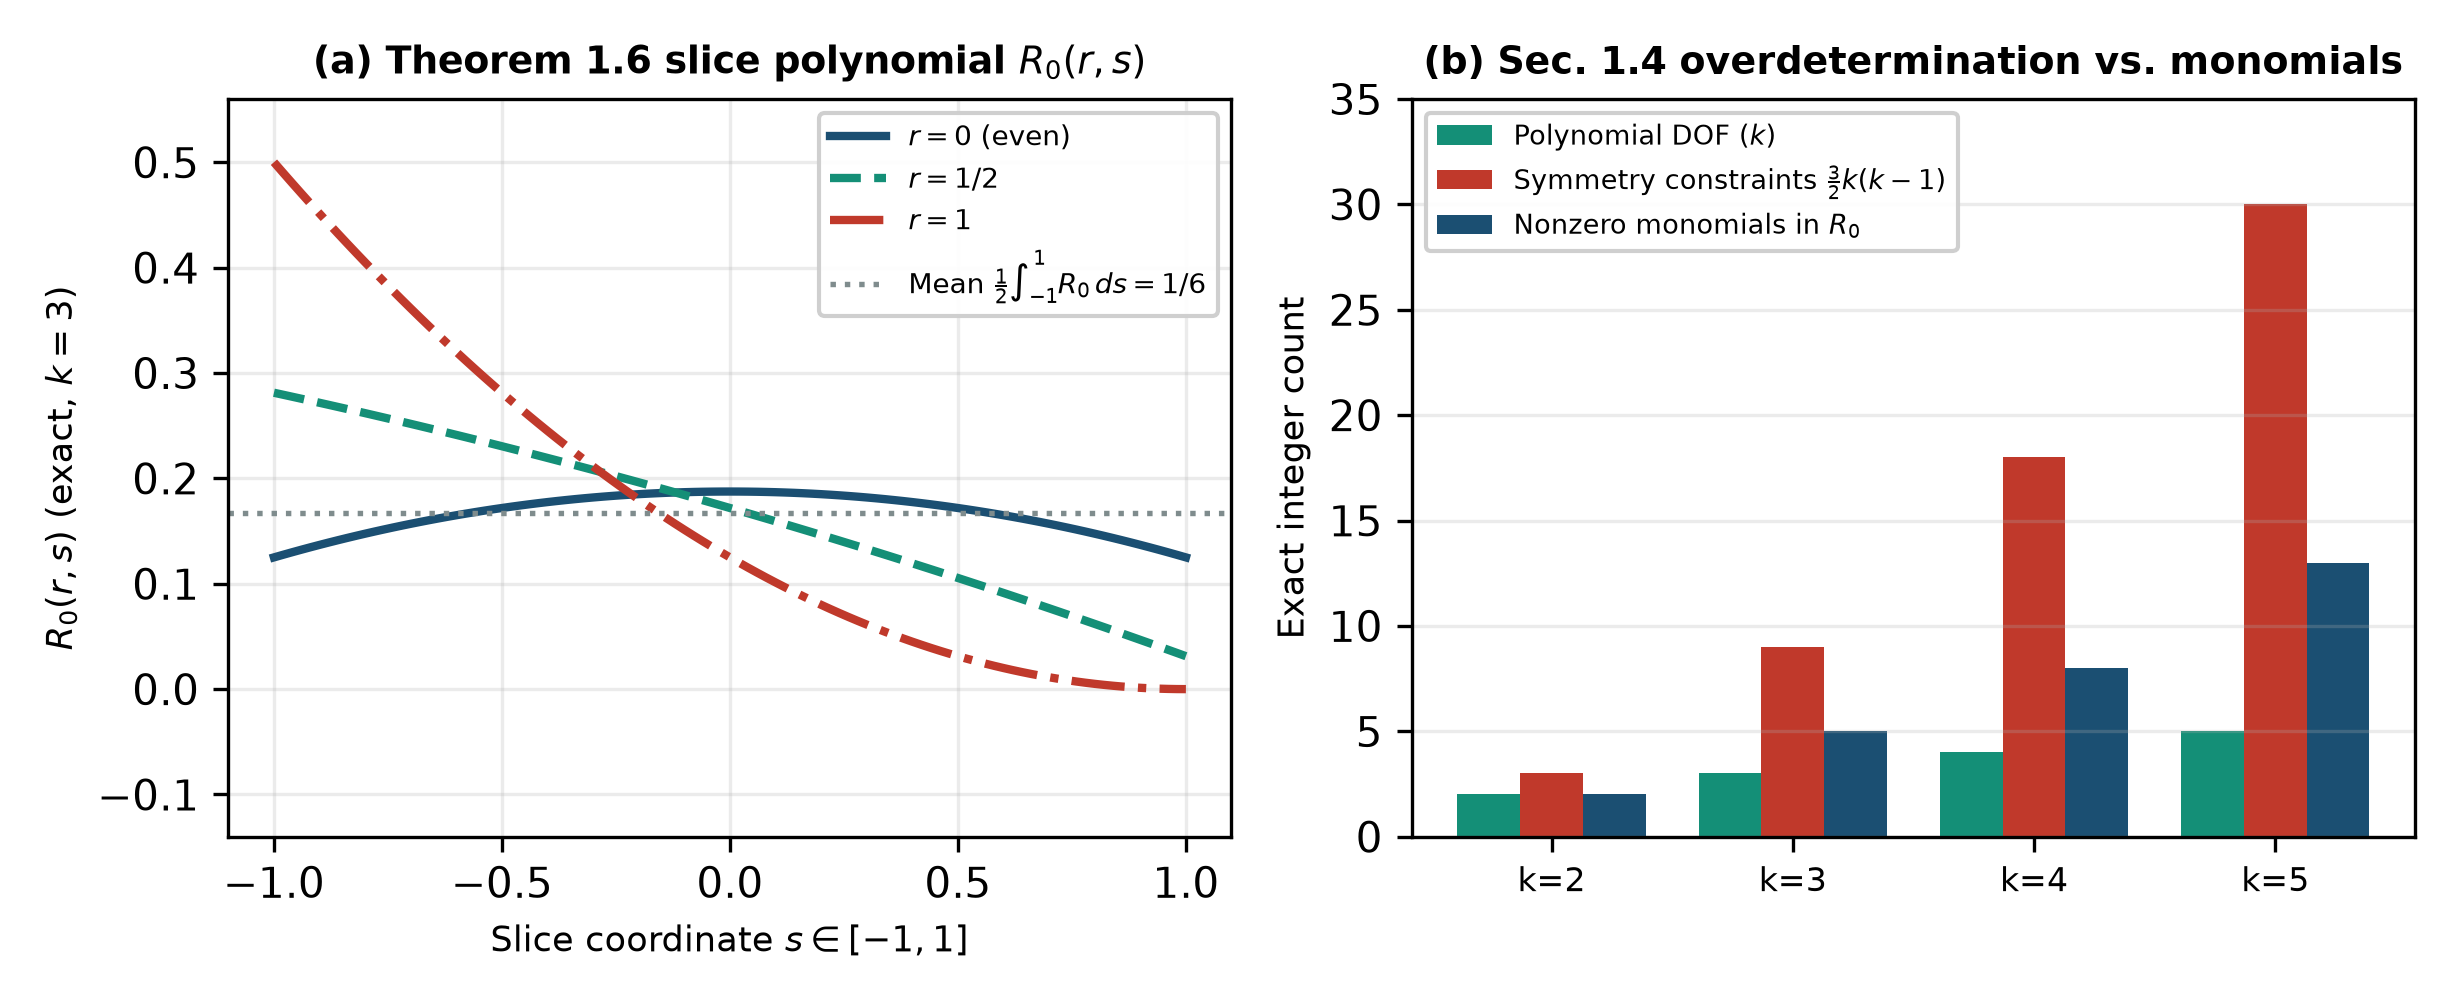
\includegraphics[width=\columnwidth]{../figures/fig1_legendre_miracle_and_overdet.png}
  \caption{(a) Exact Theorem~1.6 slice polynomial $R_0(r, s) = (3 - r^2 - 4rs - s^2 + 3r^2s^2)/16$ for $k=3$ across $r \in \{0, 1/2, 1\}$ with constant mean $1/6$ ($\int_{-1}^1 R_0\,ds = 1/3$). (b) Overdetermined symmetry constraints $\frac{3}{2}k(k-1)$ versus polynomial DOF $k$ and nonzero monomial counts for $k \in \{2,3,4,5\}$.}
  \label{fig:legendre}
\end{figure}

\paragraph{Legendre Miracle \& $m$-Basic Decompositions (Fig.~\ref{fig:legendre}).}
Mode~1 ($0.856$--$2.740\,\mathrm{ms}$) certifies $R_l(r,s)$ across $(k,l) \in \{(2,0), (3,0), (3,1), (4,1)\}$, while Dataset~1 sweeps all 14 pairs $(k,l)$ for $k \in \{2,3,4,5\}$ (up to 13 monomials, common denominator $3072$, exact marginal $1/60$, and $30$ constraints vs.\ $5$ DOF). Mode~2 ($0.079$--$0.118\,\mathrm{ms}$) certifies $k \in \{2,3\}$ unit and weighted ($m=[2,3]$, $m=[1,2,3]$) decompositions with exact $(1-x)^k$ quotients and $L^1$ costs $12$--$26$.

\begin{figure}[t]
  \centering
  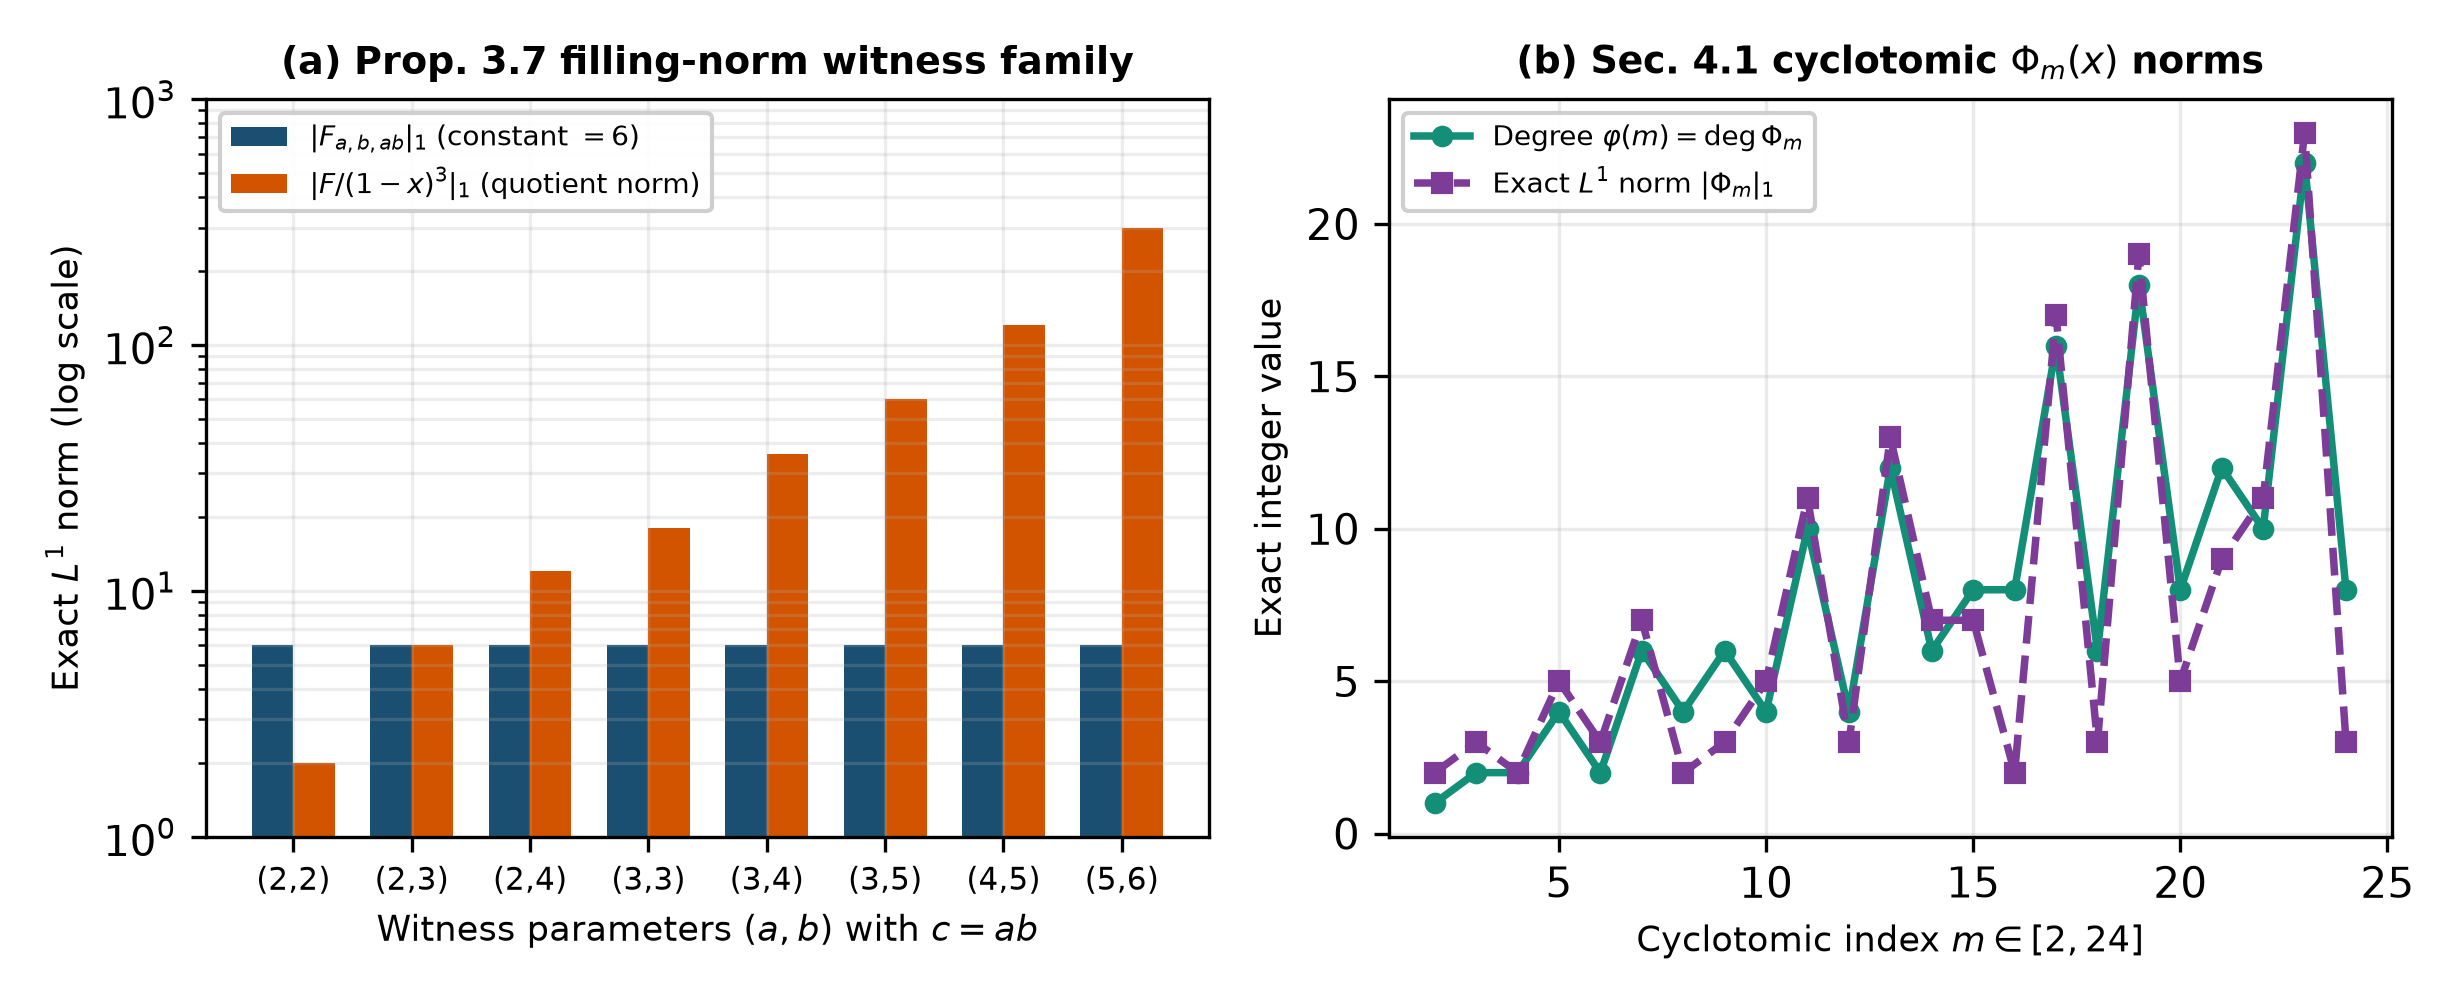
\includegraphics[width=\columnwidth]{../figures/fig2_prop37_and_cyclotomic.png}
  \caption{(a) Proposition~3.7 witness family $F_{a,b,ab}(x)$: constant $|F|_1 = 6$ versus rapidly growing $(1-x)^3$ quotient $L^1$ norm (from $2$ at $(2,2)$ to $300$ at $(5,6)$). (b) Exact cyclotomic polynomial degree $\varphi(m)$ and $L^1$ norm $|\Phi_m|_1$ across $m \in [2, 24]$.}
  \label{fig:prop37}
\end{figure}

\paragraph{Tomography, Prop.~3.7, \& Cyclotomics (Fig.~\ref{fig:prop37}).}
Mode~3 ($0.137$--$0.186\,\mathrm{ms}$) certifies 2- and 3-direction switch paths on $4\times 4$ through $7\times 7$ grids (including diagonal, anti-diagonal, and non-unimodular slope $(2,1)$ with peak entry $\le 3$). Mode~4 ($0.062$--$0.234\,\mathrm{ms}$) certifies Prop.~3.7 witnesses $(2,3,6)$ and $(3,5,15)$ ($|F|_1 = 6$, quotient degrees $4$ and $13$, exact Cramer non-vanishing) alongside complete cyclotomic factorizations for $m=12$ and $m=24$ ($|\Phi_{12}|_1 = |\Phi_{24}|_1 = 3$).

\begin{figure}[t]
  \centering
  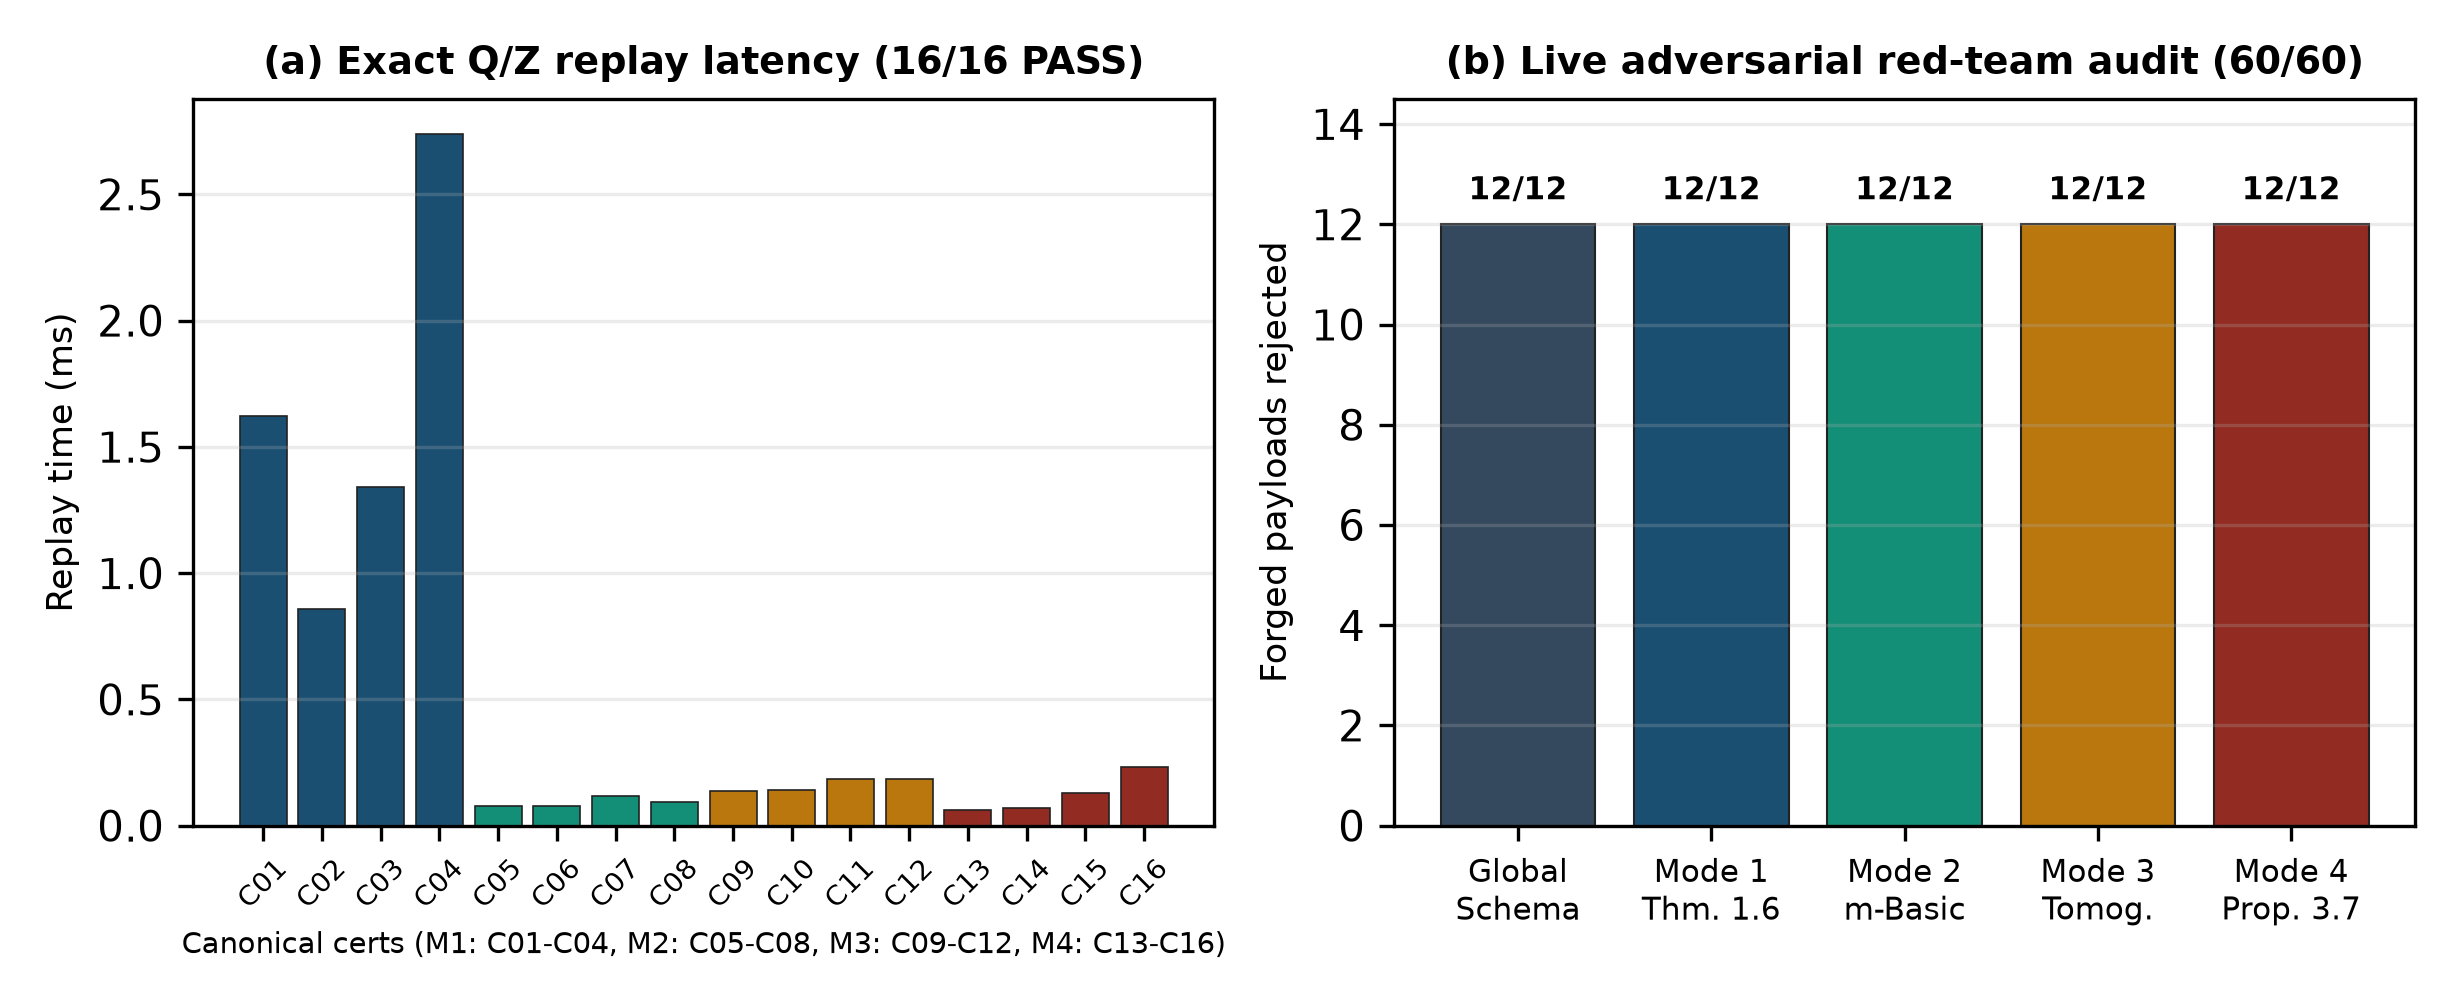
\includegraphics[width=\columnwidth]{../figures/fig3_certificate_replay_atlas.png}
  \caption{(a) Exact $\mathbb{Q}/\mathbb{Z}$ replay latency ($0.062$--$2.740\,\mathrm{ms}$) across all 16 canonical \texttt{POLY-DECOMP-CERT-1.0} certificates. (b) Live adversarial red-team audit rejecting 60/60 forged payloads across all five categories.}
  \label{fig:atlas}
\end{figure}

\paragraph{Replay Latency and 60/60 Red-Team Audit (Fig.~\ref{fig:atlas}).}
All 16 canonical certificates replay deterministically in $0.062$--$2.740\,\mathrm{ms}$ (total $8.07\,\mathrm{ms}$). The live adversarial suite (\texttt{tests/test\_suite.py}) tests 60 targeted forgeries---12 global schema/typing/canonical-rational/depth/control-char attacks plus 12 domain attacks per mode (corrupted $R_l$ monomials, unreduced rationals, trailing zeros, broken $m$-basic sums, non-primitive or collinear X-ray directions, out-of-bounds switches, $c \neq ab$, insufficient base $t$, and corrupted $\Phi_d$ coefficients)---achieving \textbf{60/60 (100\%)} rejection.

\section{Conclusion}\label{sec:conc}
We delivered a standalone, zero-floating-point verification framework for Keevash and Lim's polynomial-decomposition and reconfiguration theory~\cite{keevash2026efficient}, combining 18 zero-\texttt{sorry}, zero-\texttt{Classical.choice} Lean~4.35.0 theorems with the exact $\mathbb{Q}/\mathbb{Z}$ verifier \texttt{POLY-DECOMP-CERT-1.0}, 16 canonical certificates, and 60/60 live adversarial forgery rejections.

\bibliographystyle{plain}
\bibliography{references}
\end{document}
